\chapter{Datuen iraunkortasuna eta MongoDB}

Orain arte, inprimakiekin maneiatu ditugun datuak ez ditugu inon gorde. Express-en egindako aplikazioan ere ez gara datuen iraunkortasunaz kezkatu. Alegia, zerbitzaria itzaliz gero, memorian genituen datuak (adibidez, bezeroen izen-abizenak, helbide elektronikoak, etab.) galdu egingo ditugu. Hori ekiditeko, datuen iraunkortasuna bermatu behar dugu. Fitxategietan edo datu-baseetan gorde ditzakegu. Bigarren aukera interesgarriena da gero datu horiek modu errazean kontsultatu, iragazi edo editatu nahi baditugu. Baina datu-baseen artean sistema bat hautatzeko aukera asko ditugu. Horietako bat, MongoDB \index{MongoDB} da.

JavaScript-en programatu nahi baditugu datuen txertaketak, ezabaketak edo edizioak, oso aukera interesgarria bilakatu da MongoDB. Mongo NoSQL\index{NoSQL} motako dokumentuetara oinarritutako datu-base bat da. Mota honetako datu-baseetan ez dugu datuen eskema bat aldez aurretik derrigorrez zehaztu behar, eta datuak zuzenean txertatu ahalko ditugu JSON formatuan badaude. 

\section{MongoDB instalatu eta jaurti}

MongoDB (\textit{mongo} izenarekin askotan ezagutzen dena) Windows, Linux eta macOS sistema eragileetan instala daiteke. Bi bertsiotan banatzen da: komertziala eta doakoa (Community).  \href{https://www.mongodb.com/download-center/community}{Community server}\footnote{https://www.mongodb.com/download-center/community} doako bertsioa erabiliko dugu liburu honetan. 

Linux eta macOS-en mongo-ren konfigurazio-fitxategia bide honetan aurkituko dugu:  \hl{/usr/local/etc/mongod.conf}. Bertan zehaztuko dugu \textit{log} fitxategia non gorde nahi dugun eta zerbitzaria zer IP helbidetan jarri nahi dugun entzuten. Besterik ezeko balioak hauek dira:

\begin{lstlisting}[]
systemLog:
  destination: file
  path: /usr/local/var/log/mongodb/mongo.log
  logAppend: true
storage:
  dbPath: /usr/local/var/mongodb
net:
  bindIp: 127.0.0.1
\end{lstlisting}

Segurtasunaren aldetik interesgarria da \textit{localhost}-en (127.0.0.1 helbidean) jartzea entzuten mongodb, besterik ezeko konfigurazioan ez baitu irakurtzeko eta idazteko inolako segurtasun-neurririk indarrean, beraz, ez da batere gomendagarria \textit{bindIp} parametroan IP publiko bat jartzea.

Mongo datu-basea jaurtitzeko \hl{mongod} komandoa erabiliko dugu:

\begin{lstlisting}[numbers=none]
$ mongod --config /usr/local/etc/mongod.conf
\end{lstlisting}
 Dena ondo badoa, ez dugu inolako errorerik ikusiko. Konektatzeko, \hl{mongo}\index{mongo} komandoa landuko dugu (ikus \ref{fig:mongodb}. irudia).
 
 \begin{figure}[ht]
	\centering
\begin{tikzpicture}
\node[anchor=south west,inner sep=0] (image) at (0,0)
   {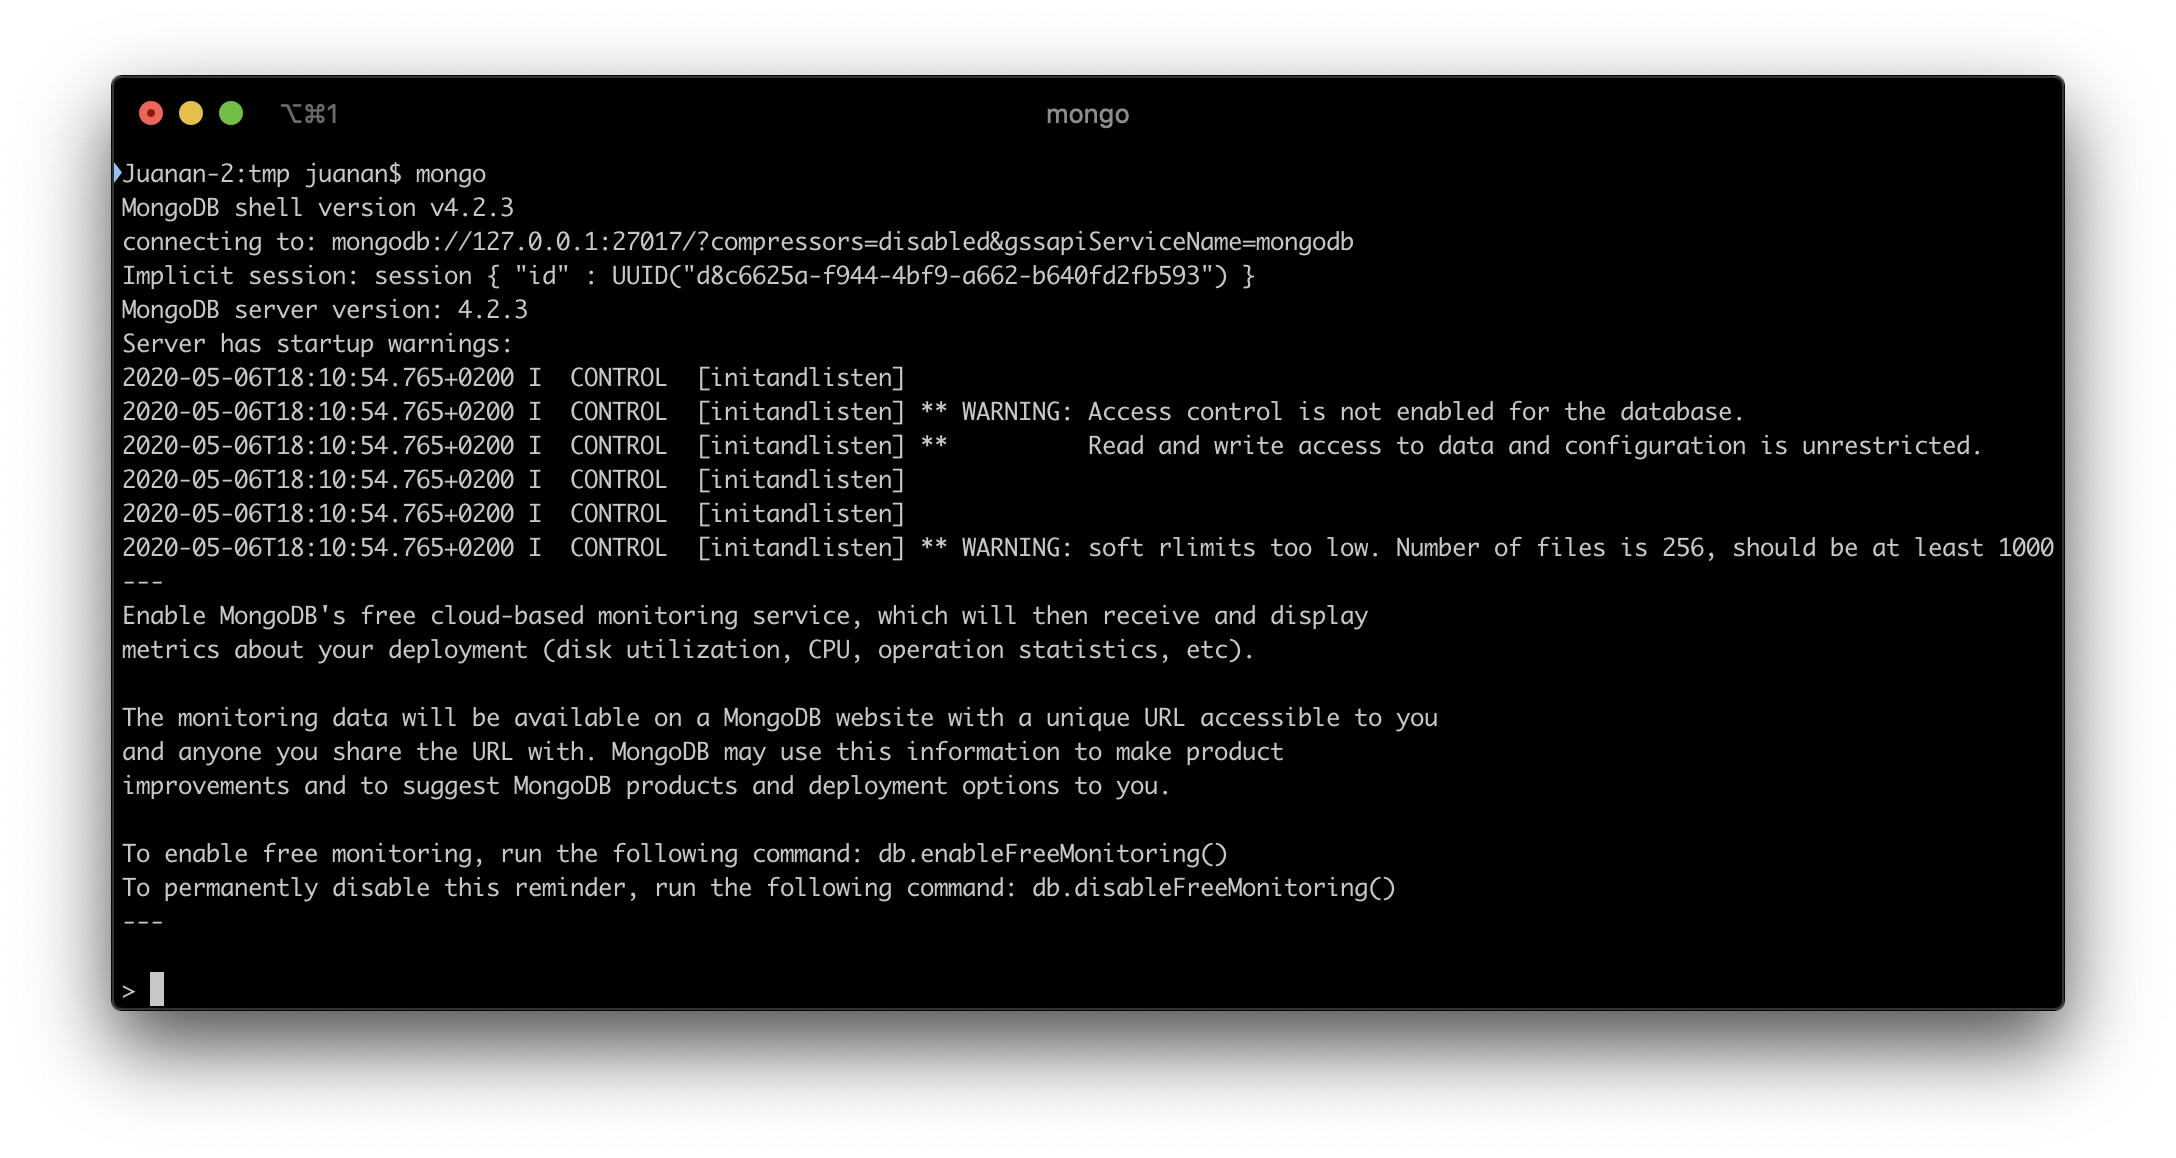
\includegraphics[trim=0cm 0cm 0cm 0cm, clip=true, width=1.0\textwidth]{img/mongo.png}};
\end{tikzpicture}
\caption{MongoDB NoSQL motako zerbitzaria jaurti ondoren lortu behar dugun mezua.}
\label{fig:mongodb}
\end{figure}

MongoDB-ra konektatu ondoren, bertan ditugun datu-baseen izenak lortzeko, \hl{show dbs}\index{show dbs} komandoa erabiliko dugu. 

\section{Datu-base berri bat ireki edo sortu}

Datu-base bat irekitzeko \hl{use}\index{use} komandoa erabiliko dugu. Adibidez, 

\begin{lstlisting}[numbers=none]
use bezeroakdb
\end{lstlisting}

Datu-basea ez bada existitzen, sortu egingo da, hasieran hutsik. Barruan dokumentuak txertatzen hasteko, bilduma bat sortu behar dugu, \hl{db.createCollection}\index{db.createCollection} komandoaz.

\begin{lstlisting}[numbers=none]
db.createCollection('bezeroak')    
\end{lstlisting}

\begin{alertinfo}{db objektua}
MongoDB-n db objektuak uneko datu-basea irudikatzen du. JavaScript objektu gisa trata dezakegu, beraz, atributuak eta metodoak izango ditu. Adibidez, db.createCollection(), db.auth(), db.getName(), db.getLastError() metodoak, edo db.bezeroak (uneko datu-basearen bezeroak bildumara apuntatzen dituena), db.constructor edo db.prototype atributuak (azken bi horiek, db JavaScript-en Object klasetik eratorritako objektu bat delako).
\end{alertinfo}

Uneko datu-basearen bildumen izenak ikusteko, \hl{show collections} komandoa erabiliko dugu.

\section{Datuak txertatzen}

Uneko datu-basean datuak txertatzeko, \hl{db.bilduma.insert} erabiliko dugu, eta parametro gisa JSON formatuan txertatu nahi ditugun dokumentuak pasatuko dizkiogu. Adibidez, aurreko ataletan landu ditugun bezeroen datuak txertatzeko:

\begin{lstlisting}[language=JavaScript, numbers=none]
db.bezeroak.insert( [    {izena: 'Ane',
        abizena: 'Uriarte',
        email: 'ane@ni.eus'},
 {
        izena: 'Jon',
        abizena: 'Juanenea',
        email: 'jon@ni.eus'
    },
    {
        izena: 'Oihane',
        abizena: 'Lete',
        email: 'oihane@ni.eus'
    }] )
\end{lstlisting}

Dena ondo badoa, \textit{mongo}-k 3 dokumentu berri txertatu ditugula esango digu (ikus \ref{fig:mongo-insert}. irudia).

\begin{figure}[ht]
	\centering
\begin{tikzpicture}
\node[anchor=south west,inner sep=0] (image) at (0,0)
   {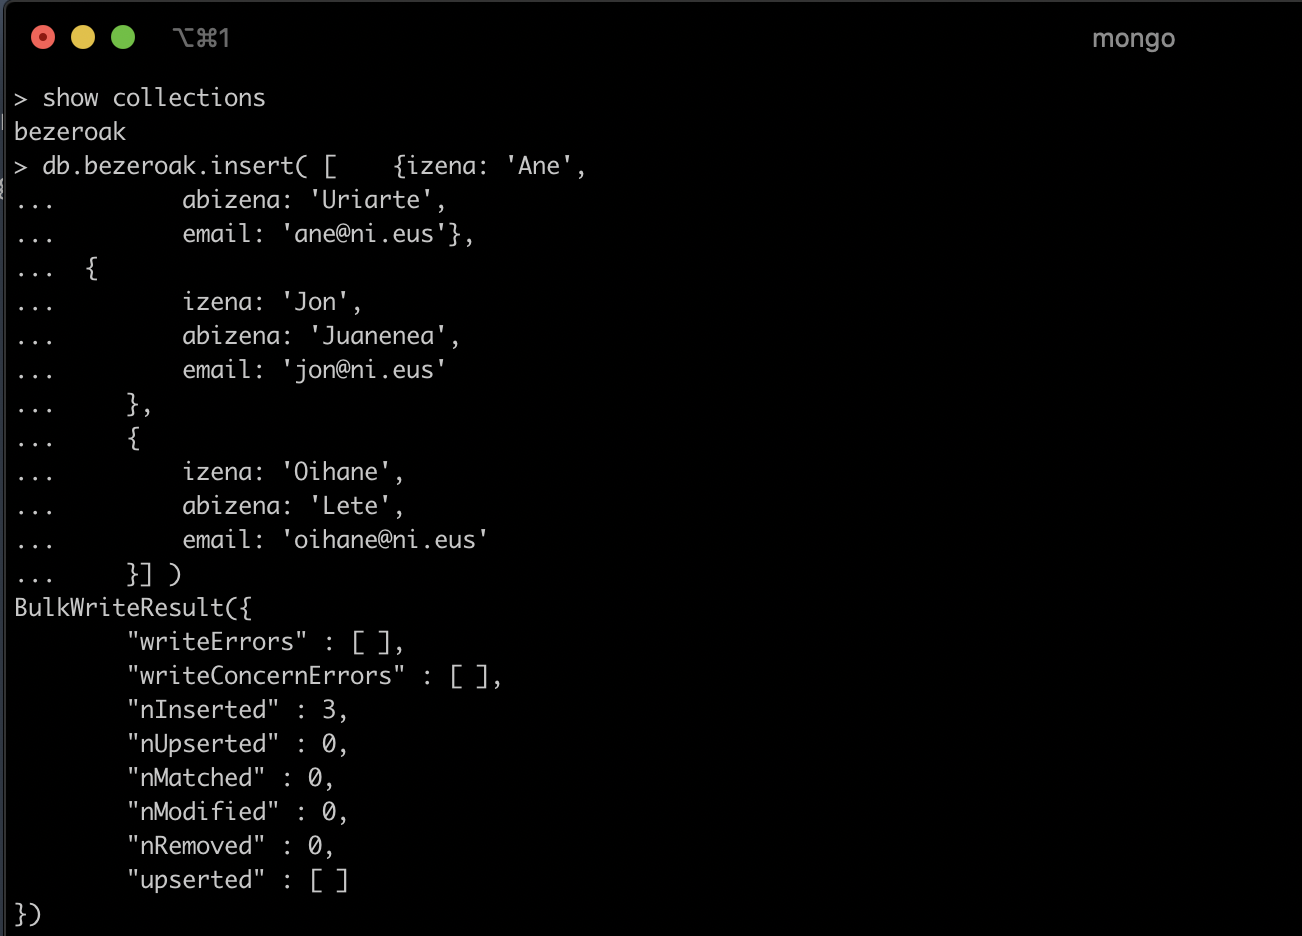
\includegraphics[trim=0cm 0cm 0cm 0cm, clip=true, width=1.0\textwidth]{img/mongo-insert.png}};
\end{tikzpicture}
\caption{Terminalarekin lan egitea ez baduzu gustukoa, Mongo-rekin lan egiteko badaude ingurune grafiko ederrak. Horietako batzuk, Studio3T (https://studio3t.com/) eta MongoDB Compass (\href{https://www.mongodb.com/products/compass}{https://www.mongodb.com/products/compass}) dira.}
\label{fig:mongo-insert}
\end{figure}

\section{Dokumentuak bilatzen}
Bilduma baten barruan dauden objektuak zerrendatu nahi baditugu, \index{db.find()}\hl{db.find()} komandoa erabiliko dugu:

\begin{lstlisting}[language=JavaScript, numbers=none]
> db.bezeroak.find()
{ "_id" : ObjectId("...08fb9"), "izena" : "Ane", "abizena" : "Uriarte", "email" : "ane@ni.eus" }
{ "_id" : ObjectId("...08fba"), "izena" : "Jon", "abizena" : "Juanenea", "email" : "jon@ni.eus" }
{ "_id" : ObjectId("...08fbb"), "izena" : "Oihane", "abizena" : "Lete", "email" : "oihane@ni.eus" }
\end{lstlisting}

Dokumentu bakoitzari, berez dituen atributuez gain, mongo-k identifikatzaile bat esleitu dio, \textit{ObjectId}\index{ObjectId} bat. 

Badago dokumentu bat bere id edo beste atributu batzuen balioen arabera bilatzeko aukera. Adibidez, id-aren edo izenaren arabera bilatzeko:

\begin{lstlisting}[language=JavaScript, numbers=none]
db.bezeroak.find(  { _id: ObjectId("5ed4c9cb64dd7facd8008fb9")  } )
{ "_id" : ObjectId("5ed4c9cb64dd7facd8008fb9"), "izena" : "Ane", "abizena" : "Uriarte", "email" : "ane@ni.eus" }

db.bezeroak.find(  { izena: "Ane"  } )
{ "_id" : ObjectId("5ed4c9cb64dd7facd8008fb9"), "izena" : "Ane", "abizena" : "Uriarte", "email" : "ane@ni.eus" }

db.bezeroak.find(  
    { izena: { $regex: /^A/ }  } 
    
{ "_id" : ObjectId("5ed4c9cb64dd7facd8008fb9"), "izena" : "Ane", "abizena" : "Uriarte", "email" : "ane@ni.eus" }
{ "_id" : ObjectId("5ed4e879ff9c131dfbe6d23b"), "izena" : "Aitor", "abizena" : "Martikorena", "email" : "aitor@ni.eus" }
{ "_id" : ObjectId("5ed4e9328a54491e39140b49"), "izena" : "Aitor", "abizena" : "Martikorena", "email" : "aitor@ni.eus" }
)
\end{lstlisting}

Azkenengo adibidean, izena A hizkiaz hasten diren bezero guztiak bilatzen ditugu (letra larriak eta xeheak ezberdintzen dira).

Adibide horretan ohartzen bagara, Aitor Martikorena birritan agertzen da. Bigarrena ezabatzeko, \hl{db.deleteOne}\index{db.deleteOne} metodoa erabil dezakegu: 

\begin{lstlisting}[language=JavaScript, numbers=none]
db.bezeroak.deleteOne( { _id: ObjectId("5ed4e9328a54491e39140b49")  }  )
\end{lstlisting}

Konexioa ixteko, \hl{Ctrl+d} sakatu edo \hl{quit()} idatziko dugu.

\section{MongoDB eta NodeJS lotzen}
MongoDB eta NodeJS lotzeko, \textit{mongojs}\index{mongojs} paketea instalatuko dugu.

\begin{lstlisting}[numbers=none]
npm install mongojs --save     
\end{lstlisting}

Orain, \href{https://mongo-js.github.io/mongojs/}{mongojs}\footnote{https://mongo-js.github.io/mongojs/} dokumentazioari jarraituz, nodetik konexio bat irekiko dugu:

\begin{lstlisting}[language=JavaScript,numbers=none]
const mongojs = require('mongojs')
const db = mongojs(connectionString, [collections])
\end{lstlisting}

Gure kasurako doitzen badugu, honela geratuko da:

\begin{lstlisting}[language=JavaScript]
const mongojs = require('mongojs')
const db = mongojs('bezeroakdb', ['bezeroak'])
\end{lstlisting}

Lerro horiek \hl{index.js} fitxategian txertatu behar ditugu.

Orain, eskuz idatzi ditugun bezeroen datuak \hl{index.js} fitxategitik ezabatu eta \textit{mongo} erabiliz jasoko ditugu. Horretarako, \hl{app.get} bidea honela utziko dugu:

\begin{lstlisting}[language=JavaScript]
app.get("/", function(req, res) {
    db.bezeroak.find( function (err, docs) {
        if (err) {
            console.log(err)
        } else {
            console.log(docs);
            res.render('index', {
                'izenburua': 'EJS probatzen',
                'bezeroak': docs
            })
        }
    })
});
\end{lstlisting}

\section{Datuen txertaketak mongo-n}

\hl{app.post} bidea moldatu egin behar dugu  inprimakitik datozen datuak mongo-n gordetzeko, \hl{db.bilduma.insert} erabiliz, lehen ikusi dugun bezala (orain parametro gisa \textit{callback} funtzio bat pasatuko diogu)

\begin{lstlisting}[language=JavaScript]
app.post('/bezeroa', function(req, res) {
    const bezeroBerria =  {
        izena : req.body.izena,
        abizena: req.body.abizena,
        email: req.body.email
    };

    console.log(bezeroBerria);
    
    db.bezeroak.insert( bezeroBerria, function(err) {
        if (err) {
            console.log(err);
        } else {
            res.redirect('/');
        }
    })
})
\end{lstlisting}

Garrantzitsua da 15. lerroan dugun \hl{res.redirect(\textquotesingle{}/\textquotesingle{})}. Horrek, datu-basean txertaketa egin ondoren, webgunearen erro-katalogora birbideratuko gaitu, \textit{app.get} bidetik sartuko gara eta bezero guztien datuak bistaratuko ditugu.


\section{Ariketa}
 
 Bezeroen datuak bistaratzean, bezero bakoitzaren izenaren ondoan, bistaratu ``Ezabatu'' eta ``Editatu'' estekak  (ikus \ref{fig:bezeroakeditatu}. irudia).
 
 
\begin{enumerate}
     \item ``Ezabatu'' estekan sakatzean, erabiltzaileari alerta bat pantailaratu behar zaio, ezabaketa egiteko ziur dagoen egiazta dezan. Baietz erantzunez gero, aukeratutako bezeroa datu-basetik ezabatu eta zerrenda eguneratuta bistaratu behar da.
     \item ``Editatu'' botoian sakatzean, bezeroen datuak (izena, abizena, helbide elektronikoa) inprimakian agertuko dira, erabiltzaileak edita ditzan. ``Gorde'' botoian sakatzean, erabiltzaile horren datuak datu-basean eguneratuko dira. Honelako kodea erabil dezakegu:
     
     \begin{lstlisting}[language=JavaScript]
     db.bezeroak.update( 
         "query": { "_id" : ObjectId("5ed4c9cb64dd7facd8008fbb")},
         "update": { 
              $set :  { 
                 "izena" : "Oihane", 
                 "abizena": "Letamendia", 
                 email: "Oihane@ni.eus"} }, function() {
                    console.log("Eguneraketa ondo burutu da";
                    // berbideraketa egin
                 });
     \end{lstlisting}
     
     
 \begin{figure}[ht]
 \centering
 \begin{tikzpicture}
 \node[anchor=south west,inner sep=0] (image) at (0,0)
    {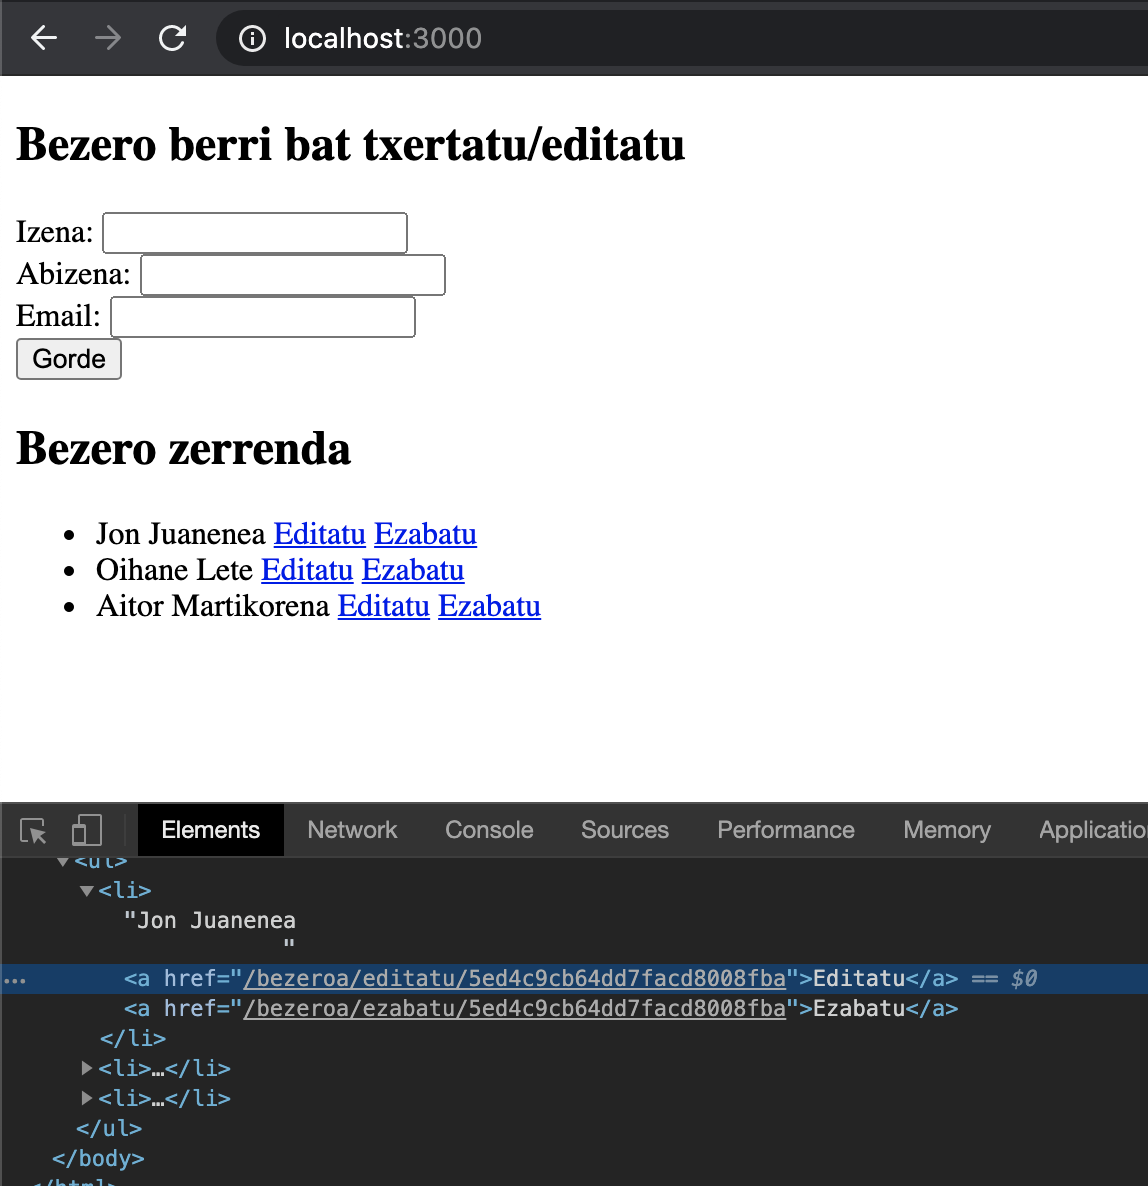
\includegraphics[trim=0cm 0cm 0cm 0cm, clip=true, width=.75\textwidth]{img/bezeroakeditatu.png}};
 \end{tikzpicture}
 \caption{Bezeroak editatu eta ezabatzeko estekak izango ditugu. Ohart zaitez esteka bakoitzean bezeroaren identifikatzailea sartu dugula.}
 \label{fig:bezeroakeditatu}
 \end{figure}
 
 \end{enumerate}  
 
 Soluzioa, \href{https://github.com/juananpe/html5liburua/blob/master/index.js}{GitHubeko biltegian} aurki dezakezu\footnote{https://github.com/juananpe/html5liburua/blob/master/index.js}.